\section{One Byte, Two Byte Exceptions}
\label{sec:vbbe21}

The one byte, two byte exceptions encoding, abbreviated to \textit{vbe21}, encodes a list of integers using one byte for each integer except for integers which cannot fit into one byte, known as \textit{exceptions}, which are encoded using two bytes. Rather than using a control code to mark where normal data and exceptions occur as in the Stream VByte codec (Section \ref{subsubsec:svb}), the exceptions are encoded at the beginning since it is expected that exceptions will occur with small probability.

The number of exceptions is written using 2 bytes, followed by the exceptions' positions in the list using 4 bytes each and the exceptions themselves using 2 bytes each.

Now, consider applying the zig-zag delta encoding to a read and then compressing using encoding $A$. Let $C_A:\Omega\to\mathbb{N}_0$ be a random variable measuring the resulting compressed size in bytes where $\Omega$ is the space of reads. Then
\begin{align*}
	C_{vbe21} &= 2 + 6X + (N - X)\\
	&= 2 + 5X + N
\end{align*}
where $N$ and $X$ are random variables measuring the read length and number of exceptions respectively.
Recall from Section \ref{subsec:prob} that the probability that a data point is greater than 255 and therefore outside the one byte range is $\sim 5\times 10^{-5}$. Thus, the expected number of exceptions is
\[ E[X] = (5 \times 10^{-5})E[N] \]
%Also, the read lengths can be modelled by the Gamma distribution $\Gamma(1.0885,0.0096)$.
where the expected read length is
\[ E[N] = 113471.4 \]
from Table \ref{tab:n}.
Then, the expected compressed size is given by
\begin{align*}
	E[C_{vbe21}] &= 2 + (2.5\times 10^{-4})E[N]+ E[N]\\
	&= 2 + 1.00025E[N]\\
	&\approx 113502.
\end{align*}
In comparison, using the Stream VByte 16 (or \textit{svb16}) encoding, the compressed size is given by
\begin{align*}
	C_{svb16} &= \lceil N/8 \rceil + 2X + (N - X)\\
	&= \lceil N/8 \rceil + X + N.
\end{align*}
Then, the expected compressed size is
\begin{align*}
	E[C_{svb16}] &= \lceil E[N]/8 \rceil + (5 \times 10^{-5})E[N] + E[N]\\
	&= \lceil E[N]/8 \rceil + 1.00005E[N]\\
	&\approx 127661\\
	&> E[C_{vbe21}].
\end{align*}
So it is clear that \textit{vbe21} saves more space than \textit{svb16}: roughly 14 KiB on average per read or an estimated 6.6 GiB for the whole data set. This is actually a very accurate estimation; see Figure \ref{fig:svb16-vbe21-zd}.

\subsection{Exceptions Encoding}

The number of exceptions per read ranges from 0 to 3616 but 99\% are between 0 and 42. The mean is $\sim$5 and the standard deviation is $\sim$18. See Table \ref{tab:ex}. Its distribution, shown in Figure \ref{fig:nex-hist}, could be nicely fitted by an exponential distribution. Notice that around 20\% of the reads have no exceptions such that their zig-zag deltas lie perfectly between 0 and 255.

\begin{table}
    \caption{\label{tab:ex} Summary statistics of the number of exceptions per read and the zig-zag delta exceptions themselves in the data.}
	\begin{tabular}{|l|m{1.8cm}|l|}
	    \hline
	    Statistic & Number of Exceptions Per Read & Exceptions\\
        \hline
		Min &0 & 256\\
		Q1 & 1& 260\\

		Q2 & 3& 266\\
		Q3 & 6& 278\\
		Max & 3616& 2317\\
\hline
		Mean & 4.8546&277.0465\\
		Mode & 0&256\\
		SD & 18.0595&36.8207\\
	\hline
    \end{tabular}
\end{table}

\begin{figure}
	\centering
% Created by tikzDevice version 0.12.3.1 on 2022-10-11 18:23:57
% !TEX encoding = UTF-8 Unicode
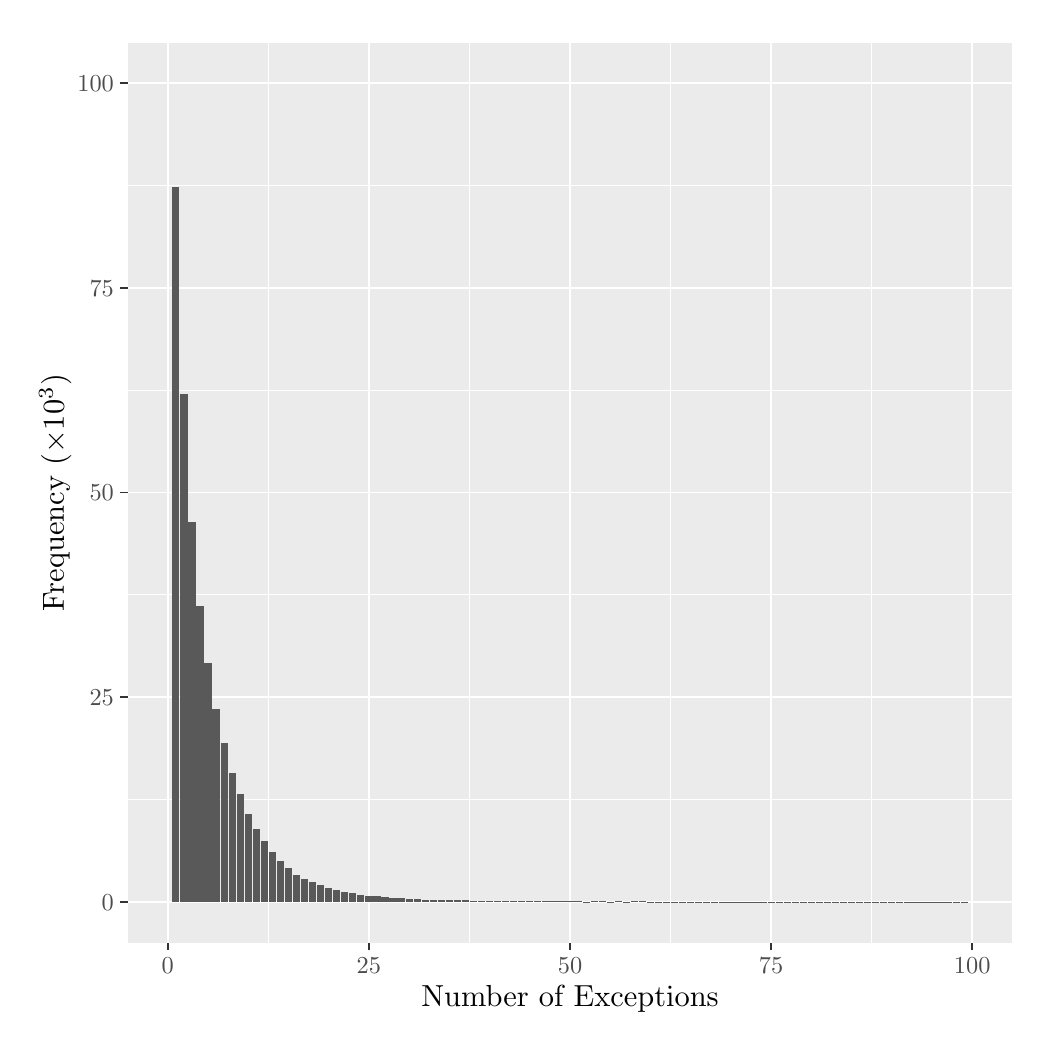
\begin{tikzpicture}[x=1pt,y=1pt]
\definecolor{fillColor}{RGB}{255,255,255}
\path[use as bounding box,fill=fillColor,fill opacity=0.00] (0,0) rectangle (361.35,361.35);
\begin{scope}
\path[clip] (  0.00,  0.00) rectangle (361.35,361.35);
\definecolor{drawColor}{RGB}{255,255,255}
\definecolor{fillColor}{RGB}{255,255,255}

\path[draw=drawColor,line width= 0.6pt,line join=round,line cap=round,fill=fillColor] (  0.00,  0.00) rectangle (361.35,361.35);
\end{scope}
\begin{scope}
\path[clip] ( 36.11, 30.69) rectangle (355.85,355.85);
\definecolor{fillColor}{gray}{0.92}

\path[fill=fillColor] ( 36.11, 30.69) rectangle (355.85,355.85);
\definecolor{drawColor}{RGB}{255,255,255}

\path[draw=drawColor,line width= 0.3pt,line join=round] ( 36.11, 82.45) --
	(355.85, 82.45);

\path[draw=drawColor,line width= 0.3pt,line join=round] ( 36.11,156.42) --
	(355.85,156.42);

\path[draw=drawColor,line width= 0.3pt,line join=round] ( 36.11,230.38) --
	(355.85,230.38);

\path[draw=drawColor,line width= 0.3pt,line join=round] ( 36.11,304.35) --
	(355.85,304.35);

\path[draw=drawColor,line width= 0.3pt,line join=round] ( 86.98, 30.69) --
	( 86.98,355.85);

\path[draw=drawColor,line width= 0.3pt,line join=round] (159.65, 30.69) --
	(159.65,355.85);

\path[draw=drawColor,line width= 0.3pt,line join=round] (232.31, 30.69) --
	(232.31,355.85);

\path[draw=drawColor,line width= 0.3pt,line join=round] (304.98, 30.69) --
	(304.98,355.85);

\path[draw=drawColor,line width= 0.6pt,line join=round] ( 36.11, 45.47) --
	(355.85, 45.47);

\path[draw=drawColor,line width= 0.6pt,line join=round] ( 36.11,119.43) --
	(355.85,119.43);

\path[draw=drawColor,line width= 0.6pt,line join=round] ( 36.11,193.40) --
	(355.85,193.40);

\path[draw=drawColor,line width= 0.6pt,line join=round] ( 36.11,267.37) --
	(355.85,267.37);

\path[draw=drawColor,line width= 0.6pt,line join=round] ( 36.11,341.34) --
	(355.85,341.34);

\path[draw=drawColor,line width= 0.6pt,line join=round] ( 50.64, 30.69) --
	( 50.64,355.85);

\path[draw=drawColor,line width= 0.6pt,line join=round] (123.31, 30.69) --
	(123.31,355.85);

\path[draw=drawColor,line width= 0.6pt,line join=round] (195.98, 30.69) --
	(195.98,355.85);

\path[draw=drawColor,line width= 0.6pt,line join=round] (268.65, 30.69) --
	(268.65,355.85);

\path[draw=drawColor,line width= 0.6pt,line join=round] (341.32, 30.69) --
	(341.32,355.85);
\definecolor{fillColor}{gray}{0.35}

\path[fill=fillColor] ( 52.24, 45.47) rectangle ( 54.86,303.76);

\path[fill=fillColor] ( 55.15, 45.47) rectangle ( 57.77,229.02);

\path[fill=fillColor] ( 58.06, 45.47) rectangle ( 60.67,182.55);

\path[fill=fillColor] ( 60.96, 45.47) rectangle ( 63.58,152.28);

\path[fill=fillColor] ( 63.87, 45.47) rectangle ( 66.49,131.71);

\path[fill=fillColor] ( 66.78, 45.47) rectangle ( 69.39,115.27);

\path[fill=fillColor] ( 69.68, 45.47) rectangle ( 72.30,103.03);

\path[fill=fillColor] ( 72.59, 45.47) rectangle ( 75.21, 92.15);

\path[fill=fillColor] ( 75.50, 45.47) rectangle ( 78.11, 84.47);

\path[fill=fillColor] ( 78.40, 45.47) rectangle ( 81.02, 77.36);

\path[fill=fillColor] ( 81.31, 45.47) rectangle ( 83.93, 71.87);

\path[fill=fillColor] ( 84.22, 45.47) rectangle ( 86.83, 67.43);

\path[fill=fillColor] ( 87.12, 45.47) rectangle ( 89.74, 63.64);

\path[fill=fillColor] ( 90.03, 45.47) rectangle ( 92.65, 60.19);

\path[fill=fillColor] ( 92.94, 45.47) rectangle ( 95.55, 57.70);

\path[fill=fillColor] ( 95.84, 45.47) rectangle ( 98.46, 55.08);

\path[fill=fillColor] ( 98.75, 45.47) rectangle (101.37, 53.84);

\path[fill=fillColor] (101.66, 45.47) rectangle (104.27, 52.65);

\path[fill=fillColor] (104.56, 45.47) rectangle (107.18, 51.51);

\path[fill=fillColor] (107.47, 45.47) rectangle (110.09, 50.42);

\path[fill=fillColor] (110.38, 45.47) rectangle (112.99, 49.62);

\path[fill=fillColor] (113.28, 45.47) rectangle (115.90, 48.95);

\path[fill=fillColor] (116.19, 45.47) rectangle (118.81, 48.54);

\path[fill=fillColor] (119.10, 45.47) rectangle (121.71, 48.05);

\path[fill=fillColor] (122.00, 45.47) rectangle (124.62, 47.58);

\path[fill=fillColor] (124.91, 45.47) rectangle (127.53, 47.40);

\path[fill=fillColor] (127.82, 45.47) rectangle (130.43, 47.26);

\path[fill=fillColor] (130.72, 45.47) rectangle (133.34, 46.87);

\path[fill=fillColor] (133.63, 45.47) rectangle (136.25, 46.79);

\path[fill=fillColor] (136.54, 45.47) rectangle (139.15, 46.48);

\path[fill=fillColor] (139.44, 45.47) rectangle (142.06, 46.53);

\path[fill=fillColor] (142.35, 45.47) rectangle (144.97, 46.31);

\path[fill=fillColor] (145.26, 45.47) rectangle (147.87, 46.29);

\path[fill=fillColor] (148.17, 45.47) rectangle (150.78, 46.20);

\path[fill=fillColor] (151.07, 45.47) rectangle (153.69, 46.11);

\path[fill=fillColor] (153.98, 45.47) rectangle (156.59, 45.98);

\path[fill=fillColor] (156.89, 45.47) rectangle (159.50, 46.01);

\path[fill=fillColor] (159.79, 45.47) rectangle (162.41, 45.94);

\path[fill=fillColor] (162.70, 45.47) rectangle (165.31, 45.80);

\path[fill=fillColor] (165.61, 45.47) rectangle (168.22, 45.91);

\path[fill=fillColor] (168.51, 45.47) rectangle (171.13, 45.81);

\path[fill=fillColor] (171.42, 45.47) rectangle (174.03, 45.73);

\path[fill=fillColor] (174.33, 45.47) rectangle (176.94, 45.84);

\path[fill=fillColor] (177.23, 45.47) rectangle (179.85, 45.73);

\path[fill=fillColor] (180.14, 45.47) rectangle (182.76, 45.74);

\path[fill=fillColor] (183.05, 45.47) rectangle (185.66, 45.74);

\path[fill=fillColor] (185.95, 45.47) rectangle (188.57, 45.67);

\path[fill=fillColor] (188.86, 45.47) rectangle (191.48, 45.69);

\path[fill=fillColor] (191.77, 45.47) rectangle (194.38, 45.65);

\path[fill=fillColor] (194.67, 45.47) rectangle (197.29, 45.68);

\path[fill=fillColor] (197.58, 45.47) rectangle (200.20, 45.71);

\path[fill=fillColor] (200.49, 45.47) rectangle (203.10, 45.59);

\path[fill=fillColor] (203.39, 45.47) rectangle (206.01, 45.66);

\path[fill=fillColor] (206.30, 45.47) rectangle (208.92, 45.63);

\path[fill=fillColor] (209.21, 45.47) rectangle (211.82, 45.59);

\path[fill=fillColor] (212.11, 45.47) rectangle (214.73, 45.60);

\path[fill=fillColor] (215.02, 45.47) rectangle (217.64, 45.58);

\path[fill=fillColor] (217.93, 45.47) rectangle (220.54, 45.62);

\path[fill=fillColor] (220.83, 45.47) rectangle (223.45, 45.60);

\path[fill=fillColor] (223.74, 45.47) rectangle (226.36, 45.55);

\path[fill=fillColor] (226.65, 45.47) rectangle (229.26, 45.57);

\path[fill=fillColor] (229.55, 45.47) rectangle (232.17, 45.55);

\path[fill=fillColor] (232.46, 45.47) rectangle (235.08, 45.56);

\path[fill=fillColor] (235.37, 45.47) rectangle (237.98, 45.56);

\path[fill=fillColor] (238.27, 45.47) rectangle (240.89, 45.55);

\path[fill=fillColor] (241.18, 45.47) rectangle (243.80, 45.52);

\path[fill=fillColor] (244.09, 45.47) rectangle (246.70, 45.53);

\path[fill=fillColor] (246.99, 45.47) rectangle (249.61, 45.57);

\path[fill=fillColor] (249.90, 45.47) rectangle (252.52, 45.54);

\path[fill=fillColor] (252.81, 45.47) rectangle (255.42, 45.54);

\path[fill=fillColor] (255.71, 45.47) rectangle (258.33, 45.53);

\path[fill=fillColor] (258.62, 45.47) rectangle (261.24, 45.51);

\path[fill=fillColor] (261.53, 45.47) rectangle (264.14, 45.53);

\path[fill=fillColor] (264.43, 45.47) rectangle (267.05, 45.50);

\path[fill=fillColor] (267.34, 45.47) rectangle (269.96, 45.52);

\path[fill=fillColor] (270.25, 45.47) rectangle (272.86, 45.53);

\path[fill=fillColor] (273.15, 45.47) rectangle (275.77, 45.53);

\path[fill=fillColor] (276.06, 45.47) rectangle (278.68, 45.51);

\path[fill=fillColor] (278.97, 45.47) rectangle (281.58, 45.53);

\path[fill=fillColor] (281.87, 45.47) rectangle (284.49, 45.53);

\path[fill=fillColor] (284.78, 45.47) rectangle (287.40, 45.50);

\path[fill=fillColor] (287.69, 45.47) rectangle (290.30, 45.50);

\path[fill=fillColor] (290.59, 45.47) rectangle (293.21, 45.49);

\path[fill=fillColor] (293.50, 45.47) rectangle (296.12, 45.51);

\path[fill=fillColor] (296.41, 45.47) rectangle (299.02, 45.50);

\path[fill=fillColor] (299.31, 45.47) rectangle (301.93, 45.53);

\path[fill=fillColor] (302.22, 45.47) rectangle (304.84, 45.51);

\path[fill=fillColor] (305.13, 45.47) rectangle (307.74, 45.51);

\path[fill=fillColor] (308.03, 45.47) rectangle (310.65, 45.51);

\path[fill=fillColor] (310.94, 45.47) rectangle (313.56, 45.50);

\path[fill=fillColor] (313.85, 45.47) rectangle (316.46, 45.50);

\path[fill=fillColor] (316.75, 45.47) rectangle (319.37, 45.53);

\path[fill=fillColor] (319.66, 45.47) rectangle (322.28, 45.50);

\path[fill=fillColor] (322.57, 45.47) rectangle (325.18, 45.50);

\path[fill=fillColor] (325.47, 45.47) rectangle (328.09, 45.51);

\path[fill=fillColor] (328.38, 45.47) rectangle (331.00, 45.50);

\path[fill=fillColor] (331.29, 45.47) rectangle (333.90, 45.51);

\path[fill=fillColor] (334.19, 45.47) rectangle (336.81, 45.50);

\path[fill=fillColor] (337.10, 45.47) rectangle (339.72, 45.49);
\end{scope}
\begin{scope}
\path[clip] (  0.00,  0.00) rectangle (361.35,361.35);
\definecolor{drawColor}{gray}{0.30}

\node[text=drawColor,anchor=base east,inner sep=0pt, outer sep=0pt, scale=  0.88] at ( 31.16, 42.44) {0};

\node[text=drawColor,anchor=base east,inner sep=0pt, outer sep=0pt, scale=  0.88] at ( 31.16,116.40) {25};

\node[text=drawColor,anchor=base east,inner sep=0pt, outer sep=0pt, scale=  0.88] at ( 31.16,190.37) {50};

\node[text=drawColor,anchor=base east,inner sep=0pt, outer sep=0pt, scale=  0.88] at ( 31.16,264.34) {75};

\node[text=drawColor,anchor=base east,inner sep=0pt, outer sep=0pt, scale=  0.88] at ( 31.16,338.31) {100};
\end{scope}
\begin{scope}
\path[clip] (  0.00,  0.00) rectangle (361.35,361.35);
\definecolor{drawColor}{gray}{0.20}

\path[draw=drawColor,line width= 0.6pt,line join=round] ( 33.36, 45.47) --
	( 36.11, 45.47);

\path[draw=drawColor,line width= 0.6pt,line join=round] ( 33.36,119.43) --
	( 36.11,119.43);

\path[draw=drawColor,line width= 0.6pt,line join=round] ( 33.36,193.40) --
	( 36.11,193.40);

\path[draw=drawColor,line width= 0.6pt,line join=round] ( 33.36,267.37) --
	( 36.11,267.37);

\path[draw=drawColor,line width= 0.6pt,line join=round] ( 33.36,341.34) --
	( 36.11,341.34);
\end{scope}
\begin{scope}
\path[clip] (  0.00,  0.00) rectangle (361.35,361.35);
\definecolor{drawColor}{gray}{0.20}

\path[draw=drawColor,line width= 0.6pt,line join=round] ( 50.64, 27.94) --
	( 50.64, 30.69);

\path[draw=drawColor,line width= 0.6pt,line join=round] (123.31, 27.94) --
	(123.31, 30.69);

\path[draw=drawColor,line width= 0.6pt,line join=round] (195.98, 27.94) --
	(195.98, 30.69);

\path[draw=drawColor,line width= 0.6pt,line join=round] (268.65, 27.94) --
	(268.65, 30.69);

\path[draw=drawColor,line width= 0.6pt,line join=round] (341.32, 27.94) --
	(341.32, 30.69);
\end{scope}
\begin{scope}
\path[clip] (  0.00,  0.00) rectangle (361.35,361.35);
\definecolor{drawColor}{gray}{0.30}

\node[text=drawColor,anchor=base,inner sep=0pt, outer sep=0pt, scale=  0.88] at ( 50.64, 19.68) {0};

\node[text=drawColor,anchor=base,inner sep=0pt, outer sep=0pt, scale=  0.88] at (123.31, 19.68) {25};

\node[text=drawColor,anchor=base,inner sep=0pt, outer sep=0pt, scale=  0.88] at (195.98, 19.68) {50};

\node[text=drawColor,anchor=base,inner sep=0pt, outer sep=0pt, scale=  0.88] at (268.65, 19.68) {75};

\node[text=drawColor,anchor=base,inner sep=0pt, outer sep=0pt, scale=  0.88] at (341.32, 19.68) {100};
\end{scope}
\begin{scope}
\path[clip] (  0.00,  0.00) rectangle (361.35,361.35);
\definecolor{drawColor}{RGB}{0,0,0}

\node[text=drawColor,anchor=base,inner sep=0pt, outer sep=0pt, scale=  1.10] at (195.98,  7.64) {Number of Exceptions};
\end{scope}
\begin{scope}
\path[clip] (  0.00,  0.00) rectangle (361.35,361.35);
\definecolor{drawColor}{RGB}{0,0,0}

\node[text=drawColor,rotate= 90.00,anchor=base,inner sep=0pt, outer sep=0pt, scale=  1.10] at ( 13.08,193.27) {Frequency ($\times 10^3$)};
\end{scope}
\end{tikzpicture}

	\caption{\label{fig:nex-hist}Histogram of the number of exceptions per read up to 100 which appears to nicely follow an exponential distribution. Values after 100 occur highly infrequently -- there are only 546 out of \num{500000} reads with more than 100 exceptions.}
\end{figure}


The exceptions range from 256 to 2317 as expected but 99\% of the exceptions do not go higher than 481. The mean and mode are $\sim$277 and 256 respectively. Refer to Table \ref{tab:ex}. The histogram of exceptions is shown in Figure \ref{fig:ex-hist}. Notably, the frequency of even-numbered exceptions is much greater than adjacent old-numbered exceptions from 256 up to $\sim$330. This is due to large positive deltas occuring more frequently than large negative deltas as previously discussed in Section \ref{subsec:stripe}.

\begin{figure}
	\centering
% Created by tikzDevice version 0.12.3.1 on 2022-10-11 17:28:28
% !TEX encoding = UTF-8 Unicode
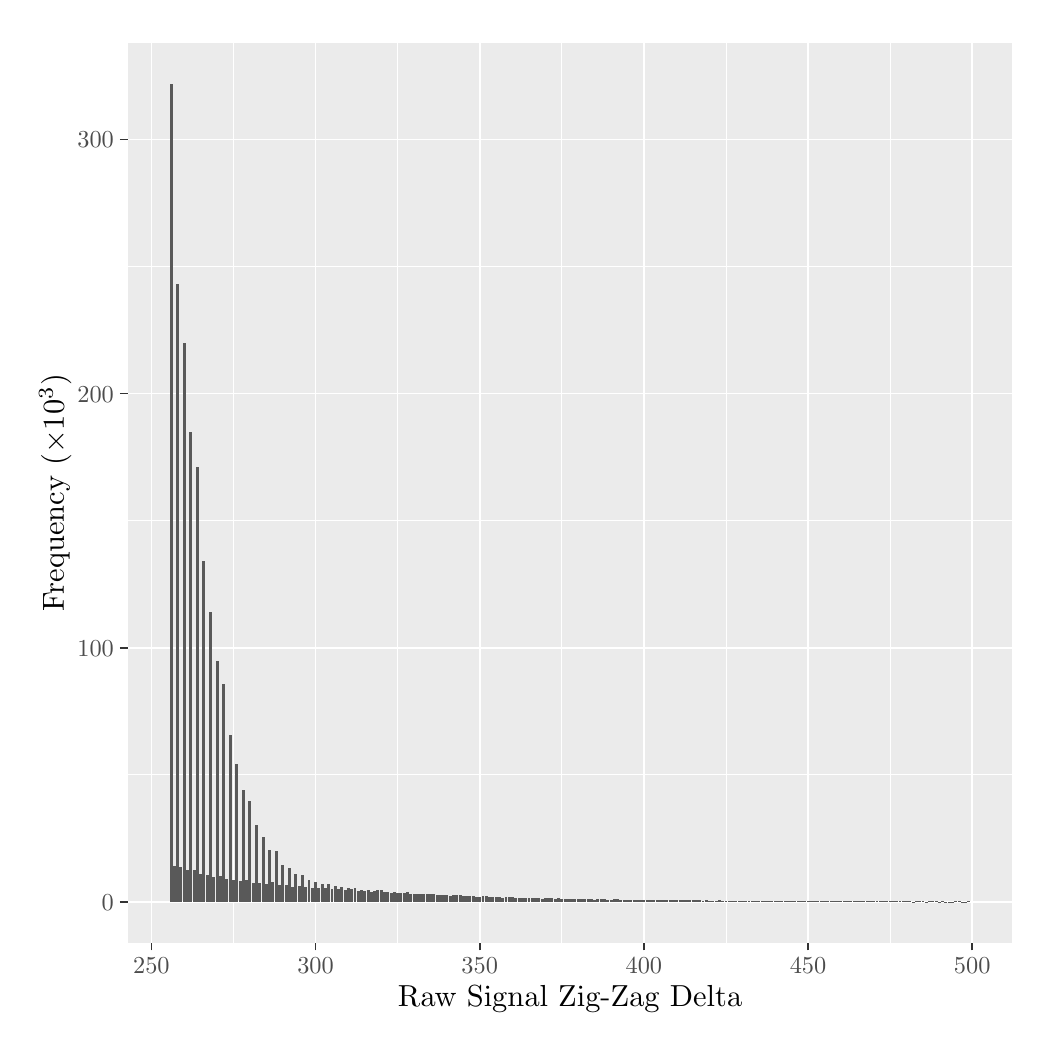
\begin{tikzpicture}[x=1pt,y=1pt]
\definecolor{fillColor}{RGB}{255,255,255}
\path[use as bounding box,fill=fillColor,fill opacity=0.00] (0,0) rectangle (361.35,361.35);
\begin{scope}
\path[clip] (  0.00,  0.00) rectangle (361.35,361.35);
\definecolor{drawColor}{RGB}{255,255,255}
\definecolor{fillColor}{RGB}{255,255,255}

\path[draw=drawColor,line width= 0.6pt,line join=round,line cap=round,fill=fillColor] (  0.00,  0.00) rectangle (361.35,361.35);
\end{scope}
\begin{scope}
\path[clip] ( 36.11, 30.69) rectangle (355.85,355.85);
\definecolor{fillColor}{gray}{0.92}

\path[fill=fillColor] ( 36.11, 30.69) rectangle (355.85,355.85);
\definecolor{drawColor}{RGB}{255,255,255}

\path[draw=drawColor,line width= 0.3pt,line join=round] ( 36.11, 91.37) --
	(355.85, 91.37);

\path[draw=drawColor,line width= 0.3pt,line join=round] ( 36.11,183.19) --
	(355.85,183.19);

\path[draw=drawColor,line width= 0.3pt,line join=round] ( 36.11,275.01) --
	(355.85,275.01);

\path[draw=drawColor,line width= 0.3pt,line join=round] ( 74.37, 30.69) --
	( 74.37,355.85);

\path[draw=drawColor,line width= 0.3pt,line join=round] (133.69, 30.69) --
	(133.69,355.85);

\path[draw=drawColor,line width= 0.3pt,line join=round] (193.01, 30.69) --
	(193.01,355.85);

\path[draw=drawColor,line width= 0.3pt,line join=round] (252.34, 30.69) --
	(252.34,355.85);

\path[draw=drawColor,line width= 0.3pt,line join=round] (311.66, 30.69) --
	(311.66,355.85);

\path[draw=drawColor,line width= 0.6pt,line join=round] ( 36.11, 45.47) --
	(355.85, 45.47);

\path[draw=drawColor,line width= 0.6pt,line join=round] ( 36.11,137.28) --
	(355.85,137.28);

\path[draw=drawColor,line width= 0.6pt,line join=round] ( 36.11,229.10) --
	(355.85,229.10);

\path[draw=drawColor,line width= 0.6pt,line join=round] ( 36.11,320.91) --
	(355.85,320.91);

\path[draw=drawColor,line width= 0.6pt,line join=round] ( 44.71, 30.69) --
	( 44.71,355.85);

\path[draw=drawColor,line width= 0.6pt,line join=round] (104.03, 30.69) --
	(104.03,355.85);

\path[draw=drawColor,line width= 0.6pt,line join=round] (163.35, 30.69) --
	(163.35,355.85);

\path[draw=drawColor,line width= 0.6pt,line join=round] (222.67, 30.69) --
	(222.67,355.85);

\path[draw=drawColor,line width= 0.6pt,line join=round] (282.00, 30.69) --
	(282.00,355.85);

\path[draw=drawColor,line width= 0.6pt,line join=round] (341.32, 30.69) --
	(341.32,355.85);
\definecolor{fillColor}{gray}{0.35}

\path[fill=fillColor] ( 51.30, 45.47) rectangle ( 52.37,341.07);

\path[fill=fillColor] ( 52.48, 45.47) rectangle ( 53.55, 58.32);

\path[fill=fillColor] ( 53.67, 45.47) rectangle ( 54.74,268.74);

\path[fill=fillColor] ( 54.86, 45.47) rectangle ( 55.92, 58.08);

\path[fill=fillColor] ( 56.04, 45.47) rectangle ( 57.11,247.36);

\path[fill=fillColor] ( 57.23, 45.47) rectangle ( 58.30, 56.94);

\path[fill=fillColor] ( 58.42, 45.47) rectangle ( 59.48,215.13);

\path[fill=fillColor] ( 59.60, 45.47) rectangle ( 60.67, 57.07);

\path[fill=fillColor] ( 60.79, 45.47) rectangle ( 61.86,202.50);

\path[fill=fillColor] ( 61.98, 45.47) rectangle ( 63.04, 55.42);

\path[fill=fillColor] ( 63.16, 45.47) rectangle ( 64.23,168.69);

\path[fill=fillColor] ( 64.35, 45.47) rectangle ( 65.42, 55.18);

\path[fill=fillColor] ( 65.53, 45.47) rectangle ( 66.60,150.14);

\path[fill=fillColor] ( 66.72, 45.47) rectangle ( 67.79, 54.37);

\path[fill=fillColor] ( 67.91, 45.47) rectangle ( 68.97,132.62);

\path[fill=fillColor] ( 69.09, 45.47) rectangle ( 70.16, 54.86);

\path[fill=fillColor] ( 70.28, 45.47) rectangle ( 71.35,124.30);

\path[fill=fillColor] ( 71.47, 45.47) rectangle ( 72.53, 53.65);

\path[fill=fillColor] ( 72.65, 45.47) rectangle ( 73.72,105.80);

\path[fill=fillColor] ( 73.84, 45.47) rectangle ( 74.91, 53.53);

\path[fill=fillColor] ( 75.03, 45.47) rectangle ( 76.09, 95.30);

\path[fill=fillColor] ( 76.21, 45.47) rectangle ( 77.28, 53.03);

\path[fill=fillColor] ( 77.40, 45.47) rectangle ( 78.47, 85.80);

\path[fill=fillColor] ( 78.58, 45.47) rectangle ( 79.65, 53.38);

\path[fill=fillColor] ( 79.77, 45.47) rectangle ( 80.84, 81.94);

\path[fill=fillColor] ( 80.96, 45.47) rectangle ( 82.03, 52.23);

\path[fill=fillColor] ( 82.14, 45.47) rectangle ( 83.21, 73.06);

\path[fill=fillColor] ( 83.33, 45.47) rectangle ( 84.40, 52.19);

\path[fill=fillColor] ( 84.52, 45.47) rectangle ( 85.58, 68.84);

\path[fill=fillColor] ( 85.70, 45.47) rectangle ( 86.77, 51.88);

\path[fill=fillColor] ( 86.89, 45.47) rectangle ( 87.96, 64.21);

\path[fill=fillColor] ( 88.08, 45.47) rectangle ( 89.14, 52.55);

\path[fill=fillColor] ( 89.26, 45.47) rectangle ( 90.33, 63.73);

\path[fill=fillColor] ( 90.45, 45.47) rectangle ( 91.52, 51.52);

\path[fill=fillColor] ( 91.64, 45.47) rectangle ( 92.70, 58.82);

\path[fill=fillColor] ( 92.82, 45.47) rectangle ( 93.89, 51.40);

\path[fill=fillColor] ( 94.01, 45.47) rectangle ( 95.08, 57.60);

\path[fill=fillColor] ( 95.19, 45.47) rectangle ( 96.26, 51.00);

\path[fill=fillColor] ( 96.38, 45.47) rectangle ( 97.45, 55.59);

\path[fill=fillColor] ( 97.57, 45.47) rectangle ( 98.64, 51.22);

\path[fill=fillColor] ( 98.75, 45.47) rectangle ( 99.82, 55.06);

\path[fill=fillColor] ( 99.94, 45.47) rectangle (101.01, 50.82);

\path[fill=fillColor] (101.13, 45.47) rectangle (102.19, 53.45);

\path[fill=fillColor] (102.31, 45.47) rectangle (103.38, 50.61);

\path[fill=fillColor] (103.50, 45.47) rectangle (104.57, 52.63);

\path[fill=fillColor] (104.69, 45.47) rectangle (105.75, 50.39);

\path[fill=fillColor] (105.87, 45.47) rectangle (106.94, 52.08);

\path[fill=fillColor] (107.06, 45.47) rectangle (108.13, 50.65);

\path[fill=fillColor] (108.25, 45.47) rectangle (109.31, 52.00);

\path[fill=fillColor] (109.43, 45.47) rectangle (110.50, 50.26);

\path[fill=fillColor] (110.62, 45.47) rectangle (111.69, 51.13);

\path[fill=fillColor] (111.80, 45.47) rectangle (112.87, 50.05);

\path[fill=fillColor] (112.99, 45.47) rectangle (114.06, 50.72);

\path[fill=fillColor] (114.18, 45.47) rectangle (115.25, 49.84);

\path[fill=fillColor] (115.36, 45.47) rectangle (116.43, 50.38);

\path[fill=fillColor] (116.55, 45.47) rectangle (117.62, 50.03);

\path[fill=fillColor] (117.74, 45.47) rectangle (118.80, 50.45);

\path[fill=fillColor] (118.92, 45.47) rectangle (119.99, 49.53);

\path[fill=fillColor] (120.11, 45.47) rectangle (121.18, 49.83);

\path[fill=fillColor] (121.30, 45.47) rectangle (122.36, 49.34);

\path[fill=fillColor] (122.48, 45.47) rectangle (123.55, 49.74);

\path[fill=fillColor] (123.67, 45.47) rectangle (124.74, 49.20);

\path[fill=fillColor] (124.86, 45.47) rectangle (125.92, 49.39);

\path[fill=fillColor] (126.04, 45.47) rectangle (127.11, 49.63);

\path[fill=fillColor] (127.23, 45.47) rectangle (128.30, 49.72);

\path[fill=fillColor] (128.41, 45.47) rectangle (129.48, 48.89);

\path[fill=fillColor] (129.60, 45.47) rectangle (130.67, 49.02);

\path[fill=fillColor] (130.79, 45.47) rectangle (131.85, 48.70);

\path[fill=fillColor] (131.97, 45.47) rectangle (133.04, 49.02);

\path[fill=fillColor] (133.16, 45.47) rectangle (134.23, 48.56);

\path[fill=fillColor] (134.35, 45.47) rectangle (135.41, 48.63);

\path[fill=fillColor] (135.53, 45.47) rectangle (136.60, 48.78);

\path[fill=fillColor] (136.72, 45.47) rectangle (137.79, 48.94);

\path[fill=fillColor] (137.91, 45.47) rectangle (138.97, 48.45);

\path[fill=fillColor] (139.09, 45.47) rectangle (140.16, 48.45);

\path[fill=fillColor] (140.28, 45.47) rectangle (141.35, 48.29);

\path[fill=fillColor] (141.46, 45.47) rectangle (142.53, 48.26);

\path[fill=fillColor] (142.65, 45.47) rectangle (143.72, 48.14);

\path[fill=fillColor] (143.84, 45.47) rectangle (144.91, 48.13);

\path[fill=fillColor] (145.02, 45.47) rectangle (146.09, 48.21);

\path[fill=fillColor] (146.21, 45.47) rectangle (147.28, 48.16);

\path[fill=fillColor] (147.40, 45.47) rectangle (148.46, 47.87);

\path[fill=fillColor] (148.58, 45.47) rectangle (149.65, 48.02);

\path[fill=fillColor] (149.77, 45.47) rectangle (150.84, 47.77);

\path[fill=fillColor] (150.96, 45.47) rectangle (152.02, 47.92);

\path[fill=fillColor] (152.14, 45.47) rectangle (153.21, 47.64);

\path[fill=fillColor] (153.33, 45.47) rectangle (154.40, 47.79);

\path[fill=fillColor] (154.52, 45.47) rectangle (155.58, 47.79);

\path[fill=fillColor] (155.70, 45.47) rectangle (156.77, 47.87);

\path[fill=fillColor] (156.89, 45.47) rectangle (157.96, 47.41);

\path[fill=fillColor] (158.07, 45.47) rectangle (159.14, 47.60);

\path[fill=fillColor] (159.26, 45.47) rectangle (160.33, 47.45);

\path[fill=fillColor] (160.45, 45.47) rectangle (161.52, 47.53);

\path[fill=fillColor] (161.63, 45.47) rectangle (162.70, 47.28);

\path[fill=fillColor] (162.82, 45.47) rectangle (163.89, 47.36);

\path[fill=fillColor] (164.01, 45.47) rectangle (165.07, 47.44);

\path[fill=fillColor] (165.19, 45.47) rectangle (166.26, 47.53);

\path[fill=fillColor] (166.38, 45.47) rectangle (167.45, 47.16);

\path[fill=fillColor] (167.57, 45.47) rectangle (168.63, 47.28);

\path[fill=fillColor] (168.75, 45.47) rectangle (169.82, 47.08);

\path[fill=fillColor] (169.94, 45.47) rectangle (171.01, 47.23);

\path[fill=fillColor] (171.13, 45.47) rectangle (172.19, 47.01);

\path[fill=fillColor] (172.31, 45.47) rectangle (173.38, 47.12);

\path[fill=fillColor] (173.50, 45.47) rectangle (174.57, 47.07);

\path[fill=fillColor] (174.68, 45.47) rectangle (175.75, 47.10);

\path[fill=fillColor] (175.87, 45.47) rectangle (176.94, 46.90);

\path[fill=fillColor] (177.06, 45.47) rectangle (178.13, 46.95);

\path[fill=fillColor] (178.24, 45.47) rectangle (179.31, 46.84);

\path[fill=fillColor] (179.43, 45.47) rectangle (180.50, 46.93);

\path[fill=fillColor] (180.62, 45.47) rectangle (181.68, 46.77);

\path[fill=fillColor] (181.80, 45.47) rectangle (182.87, 46.83);

\path[fill=fillColor] (182.99, 45.47) rectangle (184.06, 46.79);

\path[fill=fillColor] (184.18, 45.47) rectangle (185.24, 46.87);

\path[fill=fillColor] (185.36, 45.47) rectangle (186.43, 46.66);

\path[fill=fillColor] (186.55, 45.47) rectangle (187.62, 46.70);

\path[fill=fillColor] (187.74, 45.47) rectangle (188.80, 46.69);

\path[fill=fillColor] (188.92, 45.47) rectangle (189.99, 46.71);

\path[fill=fillColor] (190.11, 45.47) rectangle (191.18, 46.63);

\path[fill=fillColor] (191.29, 45.47) rectangle (192.36, 46.68);

\path[fill=fillColor] (192.48, 45.47) rectangle (193.55, 46.65);

\path[fill=fillColor] (193.67, 45.47) rectangle (194.73, 46.63);

\path[fill=fillColor] (194.85, 45.47) rectangle (195.92, 46.46);

\path[fill=fillColor] (196.04, 45.47) rectangle (197.11, 46.51);

\path[fill=fillColor] (197.23, 45.47) rectangle (198.29, 46.47);

\path[fill=fillColor] (198.41, 45.47) rectangle (199.48, 46.48);

\path[fill=fillColor] (199.60, 45.47) rectangle (200.67, 46.41);

\path[fill=fillColor] (200.79, 45.47) rectangle (201.85, 46.41);

\path[fill=fillColor] (201.97, 45.47) rectangle (203.04, 46.48);

\path[fill=fillColor] (203.16, 45.47) rectangle (204.23, 46.55);

\path[fill=fillColor] (204.34, 45.47) rectangle (205.41, 46.29);

\path[fill=fillColor] (205.53, 45.47) rectangle (206.60, 46.39);

\path[fill=fillColor] (206.72, 45.47) rectangle (207.79, 46.33);

\path[fill=fillColor] (207.90, 45.47) rectangle (208.97, 46.36);

\path[fill=fillColor] (209.09, 45.47) rectangle (210.16, 46.31);

\path[fill=fillColor] (210.28, 45.47) rectangle (211.34, 46.30);

\path[fill=fillColor] (211.46, 45.47) rectangle (212.53, 46.36);

\path[fill=fillColor] (212.65, 45.47) rectangle (213.72, 46.35);

\path[fill=fillColor] (213.84, 45.47) rectangle (214.90, 46.19);

\path[fill=fillColor] (215.02, 45.47) rectangle (216.09, 46.23);

\path[fill=fillColor] (216.21, 45.47) rectangle (217.28, 46.21);

\path[fill=fillColor] (217.40, 45.47) rectangle (218.46, 46.19);

\path[fill=fillColor] (218.58, 45.47) rectangle (219.65, 46.21);

\path[fill=fillColor] (219.77, 45.47) rectangle (220.84, 46.18);

\path[fill=fillColor] (220.95, 45.47) rectangle (222.02, 46.17);

\path[fill=fillColor] (222.14, 45.47) rectangle (223.21, 46.19);

\path[fill=fillColor] (223.33, 45.47) rectangle (224.40, 46.18);

\path[fill=fillColor] (224.51, 45.47) rectangle (225.58, 46.12);

\path[fill=fillColor] (225.70, 45.47) rectangle (226.77, 46.08);

\path[fill=fillColor] (226.89, 45.47) rectangle (227.95, 46.10);

\path[fill=fillColor] (228.07, 45.47) rectangle (229.14, 46.09);

\path[fill=fillColor] (229.26, 45.47) rectangle (230.33, 46.07);

\path[fill=fillColor] (230.45, 45.47) rectangle (231.51, 46.13);

\path[fill=fillColor] (231.63, 45.47) rectangle (232.70, 46.04);

\path[fill=fillColor] (232.82, 45.47) rectangle (233.89, 46.04);

\path[fill=fillColor] (234.01, 45.47) rectangle (235.07, 45.98);

\path[fill=fillColor] (235.19, 45.47) rectangle (236.26, 46.03);

\path[fill=fillColor] (236.38, 45.47) rectangle (237.45, 45.97);

\path[fill=fillColor] (237.56, 45.47) rectangle (238.63, 46.03);

\path[fill=fillColor] (238.75, 45.47) rectangle (239.82, 45.99);

\path[fill=fillColor] (239.94, 45.47) rectangle (241.01, 46.09);

\path[fill=fillColor] (241.12, 45.47) rectangle (242.19, 46.03);

\path[fill=fillColor] (242.31, 45.47) rectangle (243.38, 45.97);

\path[fill=fillColor] (243.50, 45.47) rectangle (244.56, 45.91);

\path[fill=fillColor] (244.68, 45.47) rectangle (245.75, 46.00);

\path[fill=fillColor] (245.87, 45.47) rectangle (246.94, 45.90);

\path[fill=fillColor] (247.06, 45.47) rectangle (248.12, 45.93);

\path[fill=fillColor] (248.24, 45.47) rectangle (249.31, 45.86);

\path[fill=fillColor] (249.43, 45.47) rectangle (250.50, 45.96);

\path[fill=fillColor] (250.61, 45.47) rectangle (251.68, 45.90);

\path[fill=fillColor] (251.80, 45.47) rectangle (252.87, 45.95);

\path[fill=fillColor] (252.99, 45.47) rectangle (254.06, 45.87);

\path[fill=fillColor] (254.17, 45.47) rectangle (255.24, 45.86);

\path[fill=fillColor] (255.36, 45.47) rectangle (256.43, 45.84);

\path[fill=fillColor] (256.55, 45.47) rectangle (257.61, 45.86);

\path[fill=fillColor] (257.73, 45.47) rectangle (258.80, 45.85);

\path[fill=fillColor] (258.92, 45.47) rectangle (259.99, 45.89);

\path[fill=fillColor] (260.11, 45.47) rectangle (261.17, 45.83);

\path[fill=fillColor] (261.29, 45.47) rectangle (262.36, 45.86);

\path[fill=fillColor] (262.48, 45.47) rectangle (263.55, 45.80);

\path[fill=fillColor] (263.67, 45.47) rectangle (264.73, 45.84);

\path[fill=fillColor] (264.85, 45.47) rectangle (265.92, 45.78);

\path[fill=fillColor] (266.04, 45.47) rectangle (267.11, 45.84);

\path[fill=fillColor] (267.22, 45.47) rectangle (268.29, 45.77);

\path[fill=fillColor] (268.41, 45.47) rectangle (269.48, 45.82);

\path[fill=fillColor] (269.60, 45.47) rectangle (270.67, 45.79);

\path[fill=fillColor] (270.78, 45.47) rectangle (271.85, 45.77);

\path[fill=fillColor] (271.97, 45.47) rectangle (273.04, 45.76);

\path[fill=fillColor] (273.16, 45.47) rectangle (274.22, 45.76);

\path[fill=fillColor] (274.34, 45.47) rectangle (275.41, 45.75);

\path[fill=fillColor] (275.53, 45.47) rectangle (276.60, 45.75);

\path[fill=fillColor] (276.72, 45.47) rectangle (277.78, 45.70);

\path[fill=fillColor] (277.90, 45.47) rectangle (278.97, 45.74);

\path[fill=fillColor] (279.09, 45.47) rectangle (280.16, 45.76);

\path[fill=fillColor] (280.28, 45.47) rectangle (281.34, 45.71);

\path[fill=fillColor] (281.46, 45.47) rectangle (282.53, 45.70);

\path[fill=fillColor] (282.65, 45.47) rectangle (283.72, 45.71);

\path[fill=fillColor] (283.83, 45.47) rectangle (284.90, 45.74);

\path[fill=fillColor] (285.02, 45.47) rectangle (286.09, 45.70);

\path[fill=fillColor] (286.21, 45.47) rectangle (287.28, 45.70);

\path[fill=fillColor] (287.39, 45.47) rectangle (288.46, 45.72);

\path[fill=fillColor] (288.58, 45.47) rectangle (289.65, 45.68);

\path[fill=fillColor] (289.77, 45.47) rectangle (290.83, 45.70);

\path[fill=fillColor] (290.95, 45.47) rectangle (292.02, 45.69);

\path[fill=fillColor] (292.14, 45.47) rectangle (293.21, 45.67);

\path[fill=fillColor] (293.33, 45.47) rectangle (294.39, 45.67);

\path[fill=fillColor] (294.51, 45.47) rectangle (295.58, 45.68);

\path[fill=fillColor] (295.70, 45.47) rectangle (296.77, 45.64);

\path[fill=fillColor] (296.89, 45.47) rectangle (297.95, 45.70);

\path[fill=fillColor] (298.07, 45.47) rectangle (299.14, 45.68);

\path[fill=fillColor] (299.26, 45.47) rectangle (300.33, 45.66);

\path[fill=fillColor] (300.44, 45.47) rectangle (301.51, 45.66);

\path[fill=fillColor] (301.63, 45.47) rectangle (302.70, 45.67);

\path[fill=fillColor] (302.82, 45.47) rectangle (303.89, 45.65);

\path[fill=fillColor] (304.00, 45.47) rectangle (305.07, 45.62);

\path[fill=fillColor] (305.19, 45.47) rectangle (306.26, 45.63);

\path[fill=fillColor] (306.38, 45.47) rectangle (307.44, 45.67);

\path[fill=fillColor] (307.56, 45.47) rectangle (308.63, 45.64);

\path[fill=fillColor] (308.75, 45.47) rectangle (309.82, 45.63);

\path[fill=fillColor] (309.94, 45.47) rectangle (311.00, 45.63);

\path[fill=fillColor] (311.12, 45.47) rectangle (312.19, 45.65);

\path[fill=fillColor] (312.31, 45.47) rectangle (313.38, 45.63);

\path[fill=fillColor] (313.49, 45.47) rectangle (314.56, 45.61);

\path[fill=fillColor] (314.68, 45.47) rectangle (315.75, 45.60);

\path[fill=fillColor] (315.87, 45.47) rectangle (316.94, 45.65);

\path[fill=fillColor] (317.05, 45.47) rectangle (318.12, 45.61);

\path[fill=fillColor] (318.24, 45.47) rectangle (319.31, 45.64);

\path[fill=fillColor] (319.43, 45.47) rectangle (320.49, 45.59);

\path[fill=fillColor] (320.61, 45.47) rectangle (321.68, 45.62);

\path[fill=fillColor] (321.80, 45.47) rectangle (322.87, 45.60);

\path[fill=fillColor] (322.99, 45.47) rectangle (324.05, 45.63);

\path[fill=fillColor] (324.17, 45.47) rectangle (325.24, 45.59);

\path[fill=fillColor] (325.36, 45.47) rectangle (326.43, 45.63);

\path[fill=fillColor] (326.55, 45.47) rectangle (327.61, 45.61);

\path[fill=fillColor] (327.73, 45.47) rectangle (328.80, 45.60);

\path[fill=fillColor] (328.92, 45.47) rectangle (329.99, 45.59);

\path[fill=fillColor] (330.10, 45.47) rectangle (331.17, 45.61);

\path[fill=fillColor] (331.29, 45.47) rectangle (332.36, 45.58);

\path[fill=fillColor] (332.48, 45.47) rectangle (333.55, 45.59);

\path[fill=fillColor] (333.66, 45.47) rectangle (334.73, 45.57);

\path[fill=fillColor] (334.85, 45.47) rectangle (335.92, 45.61);

\path[fill=fillColor] (336.04, 45.47) rectangle (337.10, 45.60);

\path[fill=fillColor] (337.22, 45.47) rectangle (338.29, 45.57);

\path[fill=fillColor] (338.41, 45.47) rectangle (339.48, 45.57);

\path[fill=fillColor] (339.60, 45.47) rectangle (340.66, 45.60);
\end{scope}
\begin{scope}
\path[clip] (  0.00,  0.00) rectangle (361.35,361.35);
\definecolor{drawColor}{gray}{0.30}

\node[text=drawColor,anchor=base east,inner sep=0pt, outer sep=0pt, scale=  0.88] at ( 31.16, 42.44) {0};

\node[text=drawColor,anchor=base east,inner sep=0pt, outer sep=0pt, scale=  0.88] at ( 31.16,134.25) {100};

\node[text=drawColor,anchor=base east,inner sep=0pt, outer sep=0pt, scale=  0.88] at ( 31.16,226.07) {200};

\node[text=drawColor,anchor=base east,inner sep=0pt, outer sep=0pt, scale=  0.88] at ( 31.16,317.88) {300};
\end{scope}
\begin{scope}
\path[clip] (  0.00,  0.00) rectangle (361.35,361.35);
\definecolor{drawColor}{gray}{0.20}

\path[draw=drawColor,line width= 0.6pt,line join=round] ( 33.36, 45.47) --
	( 36.11, 45.47);

\path[draw=drawColor,line width= 0.6pt,line join=round] ( 33.36,137.28) --
	( 36.11,137.28);

\path[draw=drawColor,line width= 0.6pt,line join=round] ( 33.36,229.10) --
	( 36.11,229.10);

\path[draw=drawColor,line width= 0.6pt,line join=round] ( 33.36,320.91) --
	( 36.11,320.91);
\end{scope}
\begin{scope}
\path[clip] (  0.00,  0.00) rectangle (361.35,361.35);
\definecolor{drawColor}{gray}{0.20}

\path[draw=drawColor,line width= 0.6pt,line join=round] ( 44.71, 27.94) --
	( 44.71, 30.69);

\path[draw=drawColor,line width= 0.6pt,line join=round] (104.03, 27.94) --
	(104.03, 30.69);

\path[draw=drawColor,line width= 0.6pt,line join=round] (163.35, 27.94) --
	(163.35, 30.69);

\path[draw=drawColor,line width= 0.6pt,line join=round] (222.67, 27.94) --
	(222.67, 30.69);

\path[draw=drawColor,line width= 0.6pt,line join=round] (282.00, 27.94) --
	(282.00, 30.69);

\path[draw=drawColor,line width= 0.6pt,line join=round] (341.32, 27.94) --
	(341.32, 30.69);
\end{scope}
\begin{scope}
\path[clip] (  0.00,  0.00) rectangle (361.35,361.35);
\definecolor{drawColor}{gray}{0.30}

\node[text=drawColor,anchor=base,inner sep=0pt, outer sep=0pt, scale=  0.88] at ( 44.71, 19.68) {250};

\node[text=drawColor,anchor=base,inner sep=0pt, outer sep=0pt, scale=  0.88] at (104.03, 19.68) {300};

\node[text=drawColor,anchor=base,inner sep=0pt, outer sep=0pt, scale=  0.88] at (163.35, 19.68) {350};

\node[text=drawColor,anchor=base,inner sep=0pt, outer sep=0pt, scale=  0.88] at (222.67, 19.68) {400};

\node[text=drawColor,anchor=base,inner sep=0pt, outer sep=0pt, scale=  0.88] at (282.00, 19.68) {450};

\node[text=drawColor,anchor=base,inner sep=0pt, outer sep=0pt, scale=  0.88] at (341.32, 19.68) {500};
\end{scope}
\begin{scope}
\path[clip] (  0.00,  0.00) rectangle (361.35,361.35);
\definecolor{drawColor}{RGB}{0,0,0}

\node[text=drawColor,anchor=base,inner sep=0pt, outer sep=0pt, scale=  1.10] at (195.98,  7.64) {Raw Signal Zig-Zag Delta};
\end{scope}
\begin{scope}
\path[clip] (  0.00,  0.00) rectangle (361.35,361.35);
\definecolor{drawColor}{RGB}{0,0,0}

\node[text=drawColor,rotate= 90.00,anchor=base,inner sep=0pt, outer sep=0pt, scale=  1.10] at ( 13.08,193.27) {Frequency ($\times 10^3$)};
\end{scope}
\end{tikzpicture}

	\caption{\label{fig:ex-hist}Histogram of the zig-zag delta exceptions up to 500. This figure is the tail of Figure \ref{fig:zd-hist}. The right and left tail of Figure \ref{fig:delta-hist} are `meshed' together during the zig-zag transformation causing the stripped pattern.}
\end{figure}


\subsection{Range Coding}

\subsection{Static Huffman}
